\documentclass{aa}
\usepackage{graphicx}
\usepackage[varg]{txfonts}
\usepackage[%draft, 
colorlinks,citecolor=blue,linkcolor=blue,urlcolor=blue]{hyperref}
\usepackage{amsmath}
\usepackage[usenames]{xcolor}
\usepackage{comment}
\usepackage{multirow}
\usepackage{chngpage}
\usepackage{lscape}
\usepackage{url}
\newcommand{\todo}[1]{{\large $\blacksquare$~\textbf{\color{red}[#1]}}~$\blacksquare$}
\newcommand{\udef}{\stackrel{\mathrm{def}}{=}}
% for tree diagram
\usepackage{forest}
\usepackage{tikz-qtree}
\usetikzlibrary{shadows,trees}

%Selma's comments
\definecolor{Wildstrawberry}{rgb}{1.0, 0.26, 0.64}
\newcommand{\SdM}[1]{{{\color{Wildstrawberry}\bf{#1}}}}
\newcommand{\newtext}[1]{{\color{ForestGreen}\bf{#1}}}

\renewcommand{\labelitemii}{$\bullet$}
\newcommand{\kms}{{\,\mathrm{km\ s^{-1}}}}
\newcommand{\Msun}{{\mathrm{M}_\odot}}

\DeclareRobustCommand{\Eqref}[1]{Eq.~\ref{#1}}
\DeclareRobustCommand{\Figref}[1]{Fig.~\ref{#1}}
\DeclareRobustCommand{\Tabref}[1]{Table~\ref{#1}}
\DeclareRobustCommand{\Secref}[1]{Sec.~\ref{#1}}

% \defcitealias{tauris:98}{TT98}
% \defcitealias{ramirez-agudelo:15}{R-A15}

\interfootnotelinepenalty=10000    % brute-forces the footnote not to break over two pages

  
\begin{document}

\title{VFTS682: a confirmed dynamical ejection?}

\author{M.~Renzo\inst{1} \and S.~E.~de~Mink\inst{1} \and \SdM{D.J. Lennon et al.} \todo{etc...}%\and
  % S.~Justham\inst{2,3} \and A.~de~Koter\inst{1} \todo{etc..order to be decided}
  .} 

\institute{{Astronomical Institute Anton Pannekoek, University of
    Amsterdam, 1098 XH Amsterdam, The Netherlands}
  % \and{School of Astronomy \& Space Science, University of the Chinese
  %   Academy of Sciences, Beijing 100012, China}
  % \and{National Astronomical Observatories, Chinese Academy of
  %   Sciences, Beijing 100012, China}
}
  
\offprints{M.~Renzo, \href{mailto:m.renzo@uva.nl}{m.renzo@uva.nl}}
\date{}
\abstract{}

\keywords{stars: kinematics, stars: runaways, stars: individual: VFTS682}
\maketitle{}

\section{Introduction}
\label{sec:intro}

\SdM{

How do massive stars form is one of the major longstanding questions in astrophysics
\citep[e.g.,][]{zinnecker:07}. Obtaining clues from observations has been challenging, because massive stars are intrinsically rare, 
%\citep[e.g.,][]{salpeter:55,kroupa:01, schneider:18}, 
evolve fast, typically reside in dense groups and they remain enshrouded in their parent cloud during the formation
process.  Major progress has been made on the theoretical side,  \citep[e.g.][]{Kuiper+2015Rosen+2016}, but the simulations are computationally very expensive. They can typically not yet resolve the length scales that are of interest to understand the 
high level of multiplicity among massive stars  \citep[][]{sana:12,sana:17}.  Understanding massive star formation, and its possible dependence on environment and metallicity, is crucial for understanding the role massive stars play within their host galaxies as sources of feedback, but also for understanding the transients that mark their death and the compact remnants they leave behind.  This is therefore a key question for the present and upcoming transient surveys \citep[e.g., LSST, BlackGem, LIGO/Virgo O3][]{}\todo{ref} which  will reveal transients associated to massive stars
evolution and death.

In has been conjectured that most, if not all, stars form in clusters \cite{lada:03}, where massive stars are thought to  form preferentially in the dense cores of clusters. In this picture, field stars are primarily the result of the dissolution of dense groups. 
 However, a significant population of massive stars has been  in relative isolation,  far from dense clusters or OB associations. The origin of this population still remains debated \citep{Lamb+2016}.   One hypothesis is that they  formed in the field, but this poses a challenge for the theories of star formation.  The alternative hypothesis is that these massive stars  formed in clusters, and then been ejected from their birth locations.  Such ejections may result from   \citep[e,g,][]{poveda:67} or from the dsiruption of binary systems by the supernova of the companion star  \citep[][]{zwicky:57, blaauw:61}. 
 
 A very interesting contribution to the debate whether or not massive stars an form in relative isolation was presented in recent years by  \cite{bestenlehner:11}, who discuss the case of the very massive star VFTS682.   This star is located in the field of the 30 Doradus region in the Large Magellanic Cloud (LMC) and was studied as part of the multi-epoch spectroscopic VLT-FLAMES Tarantula Survey (VFTS) of massive stars \citep{Evans+2011}.  With an spectral type  WNh5, an inferred initial mass of $M_\mathrm{ZAMS}=150.0^{+28.7}_{-17.4}\,M_\odot$  and a mass loss rate of  $\sim10^{-4.1\pm0.2}\,M_\odot \ \mathrm{yr}^{-1}$  \citep[][]{bestenlehner:11,schneider:18} it belongs to the most extreme objects in the region.  It is reminiscent of the very  massive stars, aka monster stars, identified by  \citet{Crowther+2010} and \citet{Crowther+2016}. 
 
Most remarkable is the location of  VFTS682.  It is located at a projected distance of $\sim$$29$\,pc from the core of the central ionizing star cluster R136.   \citet{bestenlehner:11} discuss two possibilities for the  origin of VFTS 682. Quoting directly from their abstract:  "either (i) the star either formed in situ, which would have profound implications for the formation mechanism of massive stars, or (ii) VFTS 682 is a slow runaway star that originated from the dense cluster R136, which would make it the most massive runaway known to date."  

In this study we report on our analysis of Gaia data that was was part of the second data release (DR2) \cite[][]{gaia:16,brown:18}.  We combine the radial velocity measurements from the VFTS survey \citep[][]{evans:11} with the proper motion from Gaia DR2 to reconstruct the three-dimensional velocity of VFTS682, and test the hypothesis that this star was ejected from R136. 

Our results indicate that VFTS 682 is a bona fide runaway star.  The direction an magnitude of the velocity vector is full consistent with dynamical ejection from R136.  Its inferred age is consistent with the inferred travel time. This means that the hypothesis that VFTS 682 is formed in relative isolation is rejected.  This makes  VFTS 682 the most massive runaway star known to date. 

}

% make sure to cite this in the conclusion \cite{fujii:11, banerjee:12}
\todo{missing: R136 too young for CC, cite age $\leq2$\,Myr \citep[][]{crowther:10,sabbi:12}


\section{Gaia DR2 data selection}
\label{sec:sample}

VFTS682 is labeled in the Gaia DR2
catalog\footnote{\url{https://vizier.u-strasbg.fr/viz-bin/VizieR-3?-source=I/345/gaia2}} with the
source id 4657685637907503744. The star has a
\texttt{visibility\_period} = 17, which counts how many observations have
been used to reconstruct its astrometric solution
\citep[][]{lindengren:18}. Its reported G-band
magnitude is 15.65, cf. the V-band magnitude of 16.08
\citep[][]{evans:11, bestenlehner:11}, and the reported
\texttt{astrometric\_excess\_noise} = 0. These values suggest that the Gaia
data for VFTS682 are trustworthy. However, the effective temperature
reported in Gaia DR2 is one order of magnitude lower than what found by
\cite{bestenlehner:11}, and the best fit parallax of this star is
negative. We do not use the effective temperature of the star anywhere
in this study, and we attribute the unphysical value of the parallax
to the large distance to the LMC. Our main findings do not rely on the
parallax nor the effective temperature values reported in the Gaia DR2
catalog.

%% should I really mention the line of sight velocity? Not really
%% using it...

We retrieve for VFTS682 the position in right ascension (RA) and declination (DEC)
in the IGCS frame \cite[][]{brown:18}, its
proper motion components ($\mu_\mathrm{RA}$, and $\mu_\mathrm{DEC}$,
respectively). For the radial velocity of VFTS682 and of the 30 Doradus
region as a whole, we instead use the VFTS data
as quoted in \cite{bestenlehner:11}. \Tabref{tab:vfts682} lists the values adopted throughout
this work for each of these quantities.

\begin{table}[tbp]
  \centering
    \caption{Astrometric parameters for VFTS682. The peculiar radial
    velocity $\delta v_\mathrm{rad}$ is obtained as the difference
    between the average radial velocity of the 30 Doradus region
    ($270\pm10\kms$) minus the radial velocity measured from the HeII $\lambda4686$
    line for VFTS682 ($315\pm15\kms$).}

  \begin{tabular}[htbp]{l|c|c}
    Parameter & Value & Source\\ \hline\hline
    RA \hfill[degree] &  \phantom{-}84.73 $\pm$  0.03 & \multirow{4}{*}{Gaia DR2}\\
    DEC \hfill [degree] & -69.07 $\pm$  0.05  & \\
    $\mu_\mathrm{RA}$  \hfill[$\mathrm{mas\ yr^{-1}}$] & \phantom{-0}1.84 $\pm$ 0.07 & \\
    $\mu_\mathrm{DEC}$  \hfill[$\mathrm{mas\ yr^{-1}}$] & \phantom{-0}0.78 $\pm$ 0.08& \\
    $\delta v_\mathrm{rad}$  \hfill[$\kms$] & \phantom{0}-45 $\pm$ 25 & \cite{bestenlehner:11}\\
    \hline
  \end{tabular}
  \label{tab:vfts682}
\end{table}

We define a local standard frame to derive the peculiar velocity
of VFTS682 by selecting from the Gaia DR2 catalog a sample of nearby
stars, following closely the approach of \cite{lennon:18}.
We select all the stars in a target of 0.2 degrees around R136
(NGC2070) fulfilling the following criteria. First, we require G-band
magnitude brighter than 17, correspondingly roughly to the
completeness level of the VFTS survey \citep[here we implicitly assume
G$\sim$V,][]{evans:11}. Then we require \texttt{visibility\_period} $\geq$ 5,
\texttt{astrometric\_excess\_noise} < 1, the errors on the proper
motion components to be smaller than 0.1\,$\mathrm{mas\ yr^{-1}}$,
and the proper motion components themselves to be smaller than
2\,$\mathrm{mas\ yr^{-1}}$ in absolute value. At the distance to the
LMC, $1\mathrm{mas\ yr^{-1}}\simeq250\,\kms$ \citep[e.g.,][]{lennon:18}, so the cut on the values
of the proper motions removes stars that would have projected
tangential velocities in excess of $\sim$500\,$\kms$, which are most
likely to be foreground stars. We checked that the additional
requirement of having parallaxes smaller than $2\,\mathrm{mas}$ does
not reduces further our sample. 

We calculate the averaged proper motion components for the whole
region using 
\begin{equation}
  \label{eq:mean}
  \langle \mu_i\rangle = \frac{\sum_\mathrm{stars}\frac{1}{\Delta
      \mu_i}\mu_i}{\sum_\mathrm{stars} \frac{1}{\Delta \mu_i}} \ \ , \
  \ \Delta \langle \mu_i\rangle = \frac{\sqrt{N}}{\sum_\mathrm{stars}
    \frac{1}{\Delta \mu_i}} \ \ ,
\end{equation}
where $i = \mathrm{RA}, \mathrm{DEC}$, and $\Delta \mu_i$ is the error
on the proper motion component reported by Gaia. The sums run over
all the $N=651$ stars in our selected sample. We evaluate each proper motion
component separately. For simplicity, throughout this study, we assume the same
distance of $50$\,kpc to the star \citep[][]{lebouteiller:08}, and to
the 30 Doradus region as a whole. We do not consider the error bars on
the distance determination when converting proper motions into
physical velocities. The data retrieved, and the ipython notebook used for the analysis
presented here will be made available at \todo{probably git repo on bitbucket?}. 

\section{The kinematics of VFTS682}
\label{sec:results}

\subsection{Is it a runaway star?}
\label{sec:runaway}
We first address the question of whether VFTS682 is a typical star
from the kinematic point of view, or whether it is a runaway star with
a significantly large peculiar velocity compared to its surrounding population. The former is what should
be expected if it formed where we observe it today, in relative
isolation from other massive stars.

Using the 651 stars selected as described in \Secref{sec:sample} (a
subset is shown in blue in \Figref{fig:main}), we find averaged proper motion components of
$\langle\mu_\mathrm{RA}\rangle = 1.683\pm0.002\,\mathrm{mas\ yr^{-1}}$ and
$\langle\mu_\mathrm{DEC}\rangle =
0.672\pm0.003\,\mathrm{mas\ yr^{-1}}$. We note that these values are
in good agreement with what found by \cite{lennon:18}. Subtracting these values from the
proper motions of VFTS682 (see \Tabref{tab:vfts682}), we obtain the
components of proper motion of the star relative to the surrounding region
$\mu_\mathrm{RA} = 0.16\pm 0.07\,\mathrm{mas\ yr^{-1}}$ and $\mu_\mathrm{DEC} =
0.11\pm 0.08\,\mathrm{mas\ yr^{-1}}$. We note that the error budget is
dominated by the errors on the proper motion components of VFTS682.

These can be converted in the
the components of the relative transverse velocity $\delta v_\mathrm{RA}=38\pm17\,\kms$,
$\delta v_\mathrm{DEC}=26\pm19\,\kms$, assuming a distance of
50\,kpc (we do not account for the uncertainty in the distance
estimate when propagating errors). The radial velocity from
\cite{bestenlehner:11} then gives the third component along
the line of sight, allowing us to calculate the three-dimensional
peculiar speed of the star:

\begin{equation}
  \label{eq:speed_around}
  v_\mathrm{pec} = \sqrt{\left(\delta v_\mathrm{RA}\right)^2
    +\left(\delta v_\mathrm{DEC}\right)^2+\left(\delta
      v_\mathrm{rad}\right)^2} = 64 \pm 21 
  \, \kms \ .
\end{equation}
This value for the three-dimensional speed of VFTS682 with respect the
surrounding stars make it the most massive ``bona fide'' runaway star
known to date.

\subsection{Does it come from the R136 cluster?}
\label{sec:r136_origin}

The red arrow in \Figref{fig:main} shows the proper motion of VFTS682
relative to the region, and the lighter red arrows show the possible
range of directions within the uncertainties in the measured proper
motion. It is clear that the most likely origin of the star is R136,
as predicted by \cite{fujii:11, banerjee:12}.

%\subsection{Kinematic age}

We can therefore consider the kinematic age for this star assuming
that it originates from the cluster,

\begin{equation}
  \label{eq:kin_age}
  \tau_\mathrm{kin} = \frac{d_\parallel}{v_\parallel} =
  \frac{29\,\mathrm{pc}}{46\,\kms} \simeq 0.63\, \mathrm{Myr} \ \ ,
\end{equation}
where $d_\parallel =29$\,pc is the projected distance from VFTS682 to
the core of R136 \citep[][]{bestenlehner:11}, $v_\parallel \equiv \sqrt{\left(\delta v_\mathrm{RA}\right)^2
    +\left(\delta v_\mathrm{DEC}\right)^2} =46\pm
17\,\kms$ is the speed of the star relative to the cluster projected on the sky, obtained
using the relative proper motion components calculated in
\Secref{sec:runaway}, and we use the approximation $1 \kms \simeq 1
\mathrm{pc \ Myr^{-1}}$.

The kinematic age $\tau_\mathrm{kin}$ is smaller than the apparent age
of the star age $1.0\pm 0.2$\,Myr from \cite{schneider:18}, which
corroborates the idea that the star is the result of a dynamical
ejection. 

\begin{figure}[htbp]
  \centering
  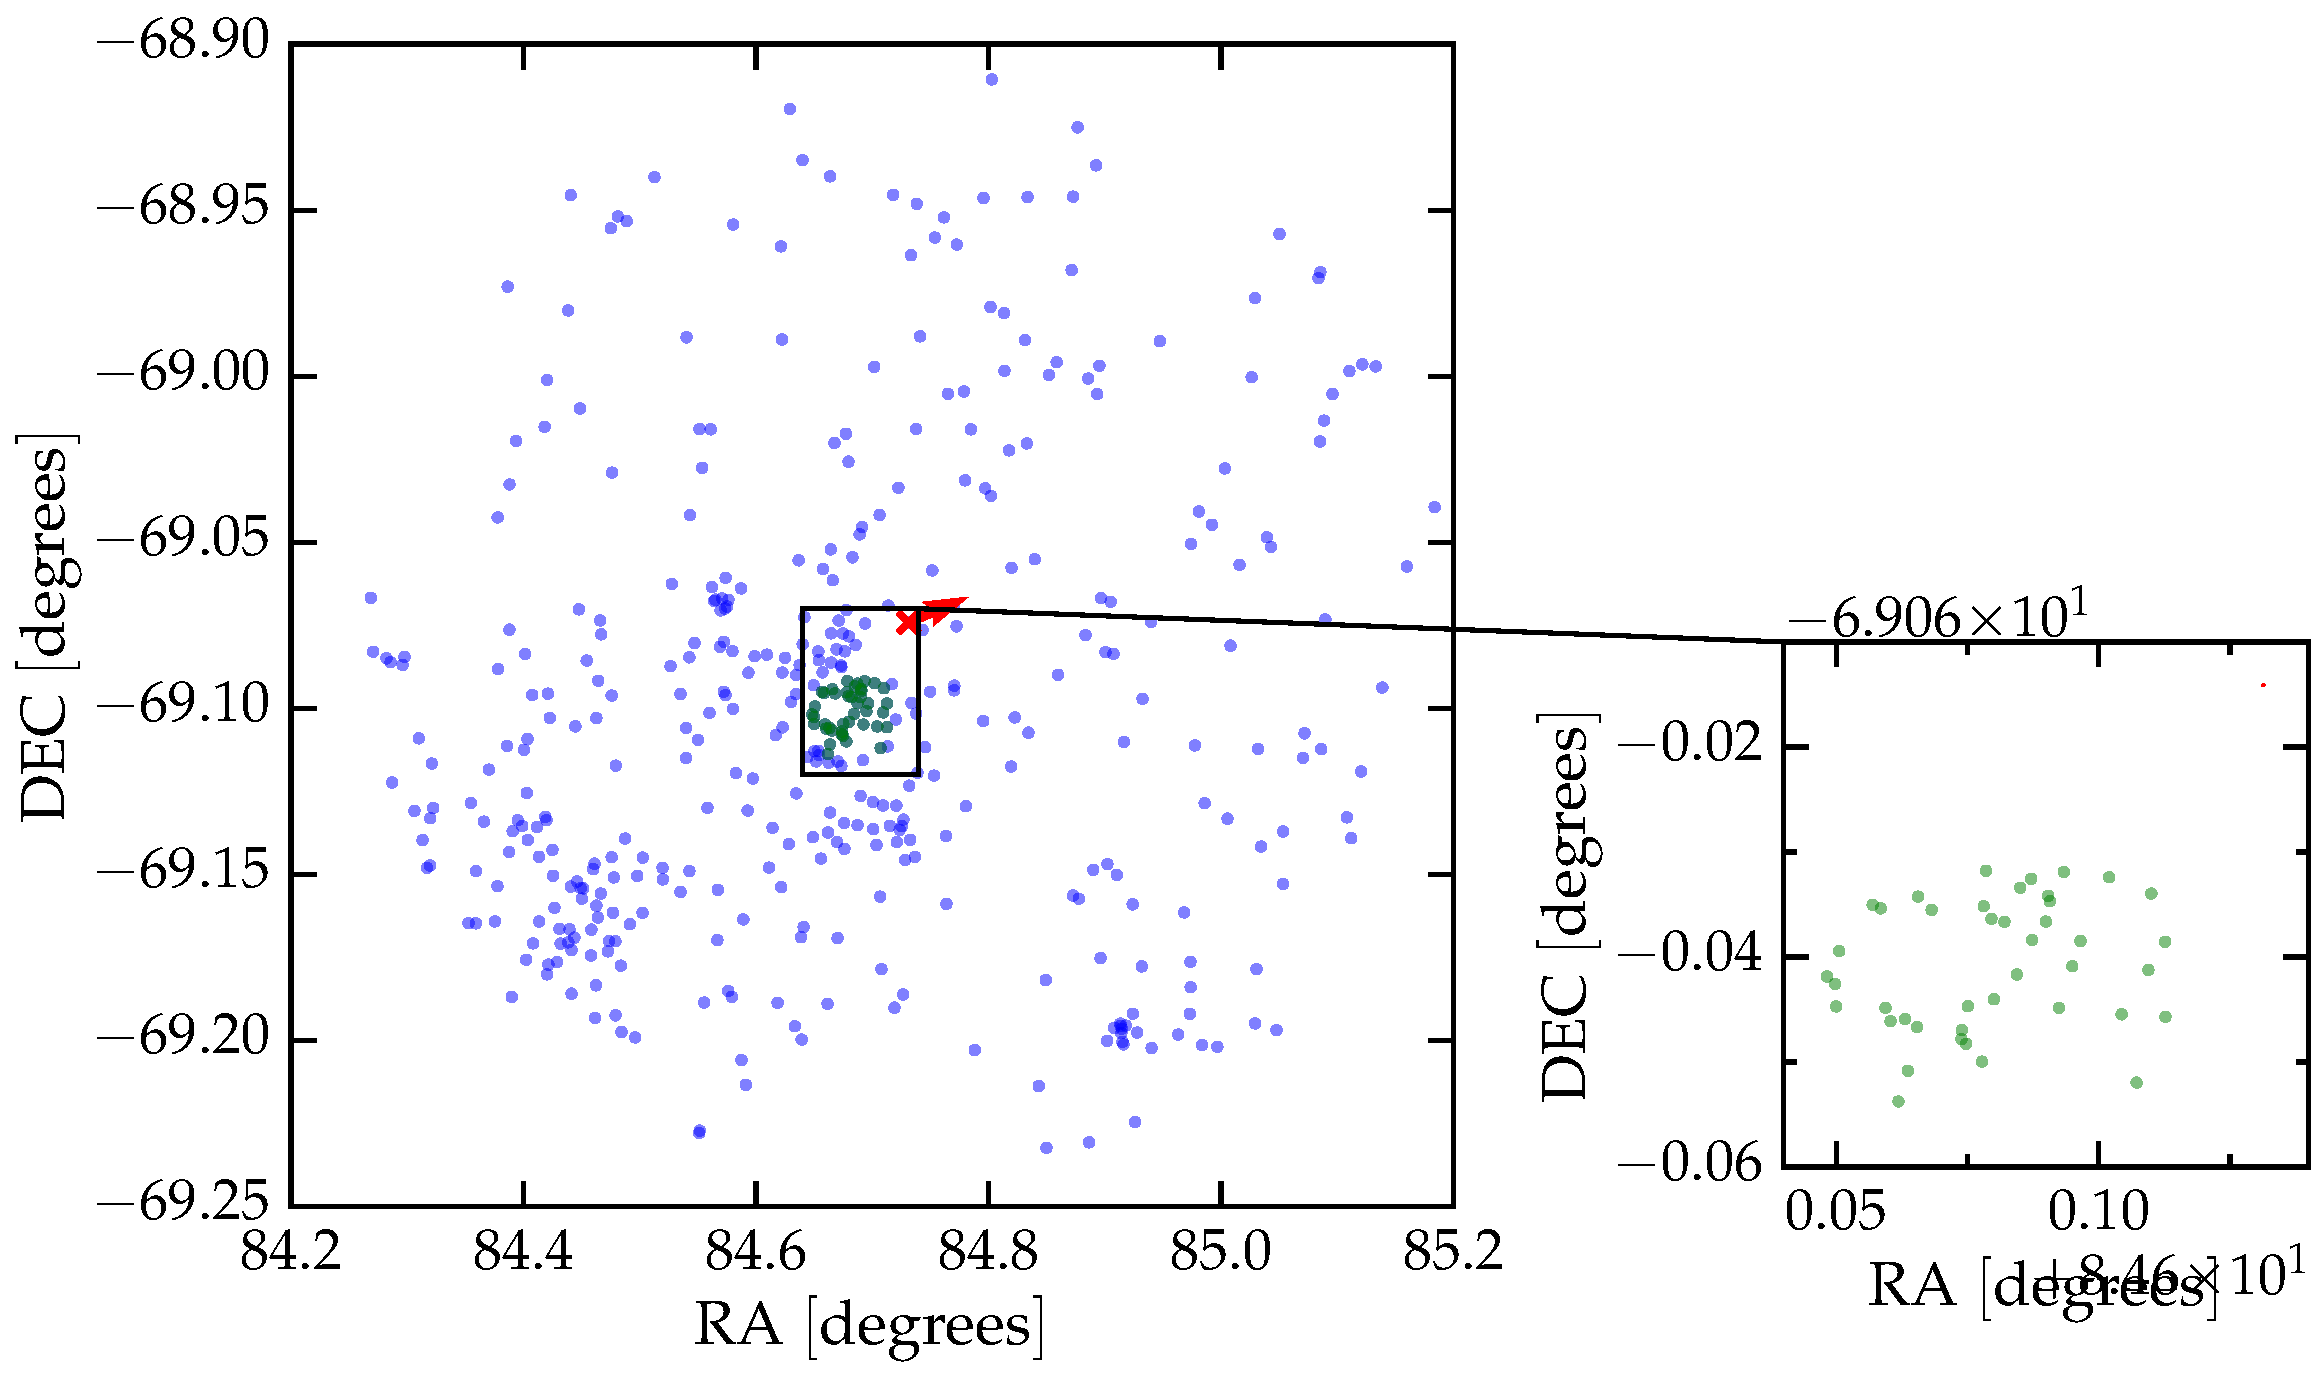
\includegraphics[width=0.5\textwidth]{./figures/main_plot}  
  \caption{The red solid arrow indicates the proper motion of VFTS682
    relative to the region, starting from the present day position of
    the star. The semi-transparent arrows indicate the possible
    directions of projected motion within the errors, and are extended
    backwards to illustrate the uncertainty on the origin of the
    star. Blue stars
    are a subset of those we use to define the local rest frame. \todo{load color picture on background}}
  \label{fig:main}
\end{figure}

\section{Discussion}
\label{sec:discussion}

Based on our results, we can claim that VFTS682 is the most massive
runaway known to date, with a peculiar three-dimensional spatial
velocity of $\sim$$60\,\kms$. This means that isolated star formation is
\emph{not} required to explain this star. Its proper motion suggests that it was ejected from the cluster R136
$\sim$$0.6$\,Myr ago. Because of the exceptionally large mass
of this star, this raises the question of which stars must populate
the core of the cluster.

Dynamical ejections due to N-body interactions typically (although, not necessarily) eject the least
massive star among those interacting \todo{ref}. This means that, just
based on the kinematic properties of VFTS682, we would expect several
stars with initial masses larger than $\sim$$150\,M_\odot$ in the
cluster R136.
This can be considered an independent confirmation of the detection
of extremely massive stars by \cite{crowther:10} in the core of the
cluster. The projected rotational equatorial velocity of VFTS682
reported by \cite{schneider:18} is $v\sin(i)<200\,\kms$, which is in
line with the average rotation rate of massive stars in the region
\citep[][]{ramirez-agudelo:15}. This suggests that VFTS682 has not
experienced binary interactions, nor it will, since the multi-epoch
data of the VFTS survey rule out the presence of a companion at
present day. Moreover, the spectral type of VFTS682
\citep[WNh5,][]{bestenlehner:11} is the same as R136a1-a3, i.e.~the
three most massive stars detected in the core of the cluster by
\cite{crowther:10}. Therefore,
VFTS682 might be an ideal target to constrain the stellar physics of
stars with masses well above $\sim100\,M_\odot$: its isolation makes
it an easier target for observations compared to the similar stars present the crowded core of R136.

The similarities between VFTS682 and the WNh5 stars in the core of
R136 are also in agreement with the ``bully binary'' model of
\cite{fujii:11}. Based on their numerical results, they suggested that
early in the evolution of a cluster, dynamical interactions form an extremely
massive binary, which then tightens its orbit by ejecting other stars passing
by. Interpreting our results for VFTS682 through the lens of their simulations
suggests the presence of a binary with total mass
$M_1+M_2\gtrsim 300\,M_\odot$ in the core of the cluster. Such bully
binary could be R145 according to \cite{fujii:11}.

The kinematic age of VFTS682 puts an
upperlimit to the timescale to form such ``bully binary'' in
R136. The cluster must have been at the very beginning of its
evolution, given the age estimate of $\lesssim 2$\,Myr
\cite{crowther:10,sabbi:12} and the kinematic age of VFTS16.

\todo{check \cite{banerjee} and rewrite next paragraph, they
  have stuff} Unfortunately, their simulations did not include stars more
massive than $100\,M_\odot$, so it is difficult to predict, based on
the existence of VFTS682, how many other stars should have been
ejected from the cluster already and what is their mass
distribution. A comprehensive study of the kinematic properties of the
large sample of stars with extremely large inferred masses visible
around R136 is encouraged.  

\cite{lennon:18} have carried out a similar study on VFTS16, another
massive star ($\sim90\,M_\odot$) in the 30 Doradus region, previously
known to be a runaway from the value of
its radial velocity. They also concluded that VFTS16 is 
the result of a dynamical ejection from the R136 cluster. 
The value of $\tau_\mathrm{kin}\simeq0.63$\,Myr we find for VFTS682 (see \Secref{sec:r136_origin}) is smaller
than the corresponding value for VFTS16: \cite{lennon:18} inferred a kinematic age of
$\sim$1.5\,Myr, possibly in tension with the apparent age of that star. This means that the more
massive VFTS682 was ejected later than VFTS16 from the same cluster.



\begin{itemize}
\item is R136 a single young cluster or a merger
\item estimate the influence of the gravitational potential of R136,
  what is its total mass and relaxation time?
\item another important thing missing: with vsini(i)<200, completely average, there is no reason to think it's a CHE, contrary to the way they estimate the age in Bestenlehner:11
\end{itemize}


\bibliographystyle{aa}
\bibliography{bibliography/vfts682}

\begin{acknowledgements}
  We are grateful to S.~Torres for extremely useful discussions on the
  Gaia DR2 dataset, and to M.~C.~Ramirez-Tannus for invaluable help.
  The background image of \Figref{fig:main} is based on observations
  made with ESO Telescopes at the La Silla Observatory under programme
  ID 076.C-0888, processed and released by the ESO VOS/ADP group.
  This research made use of APLpy, an open-source plotting package for Python \citep[][]{robitaille:12}.
\end{acknowledgements}
\end{document}




%%% Local Variables:
%%% mode: latex
%%% TeX-master: t
%%% End:
